\chapter{Návrh architektury systému}

Systém CI pod sebou bude spravovat několik Runnerů, každý Runner v~sobě bude spouštět jednotlivé exekutory.
Komunikace bude probíhat přes API.
Jakákoliv funkcionalita by měla být zprvu naimlementovaná jako API endpoint a až pak zavedena do systému.

\section{Části systému}

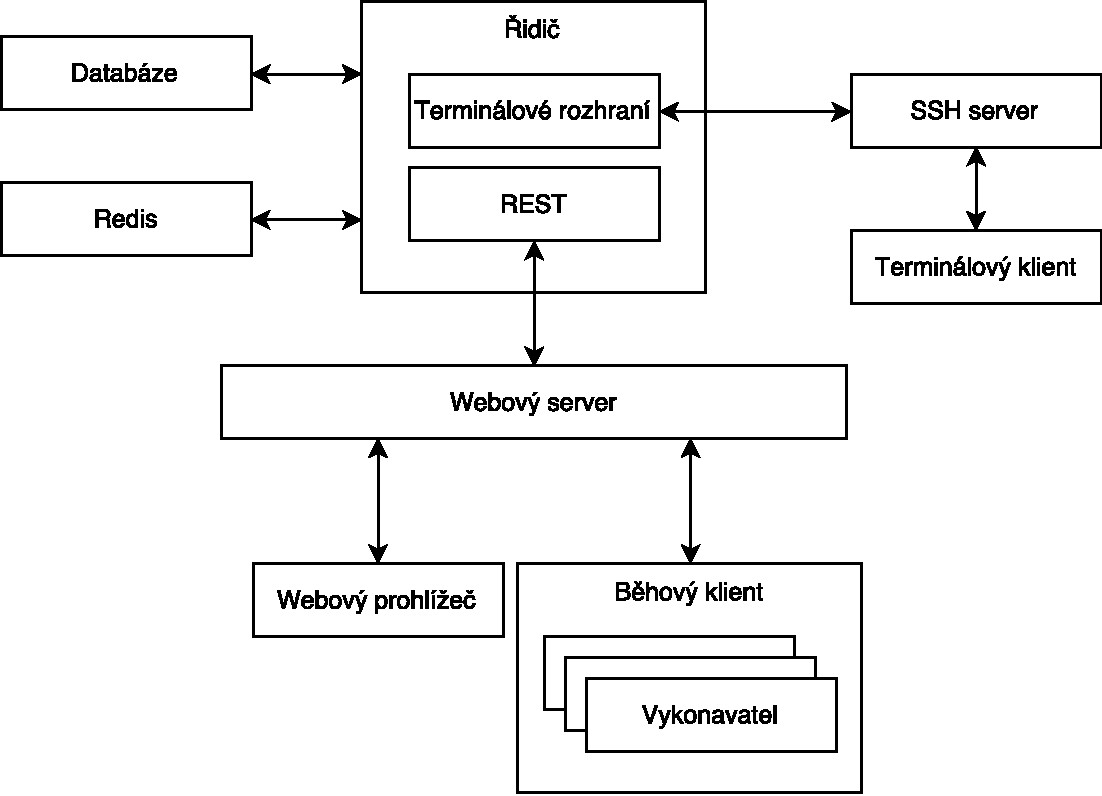
\includegraphics[max width=\linewidth]{architektura_piper.pdf}

\subsection{Řidič}

Zajišťuje komunikaci s~uživatelem, informačním rozhraním a Runnery na pevně daném protokolu.
Řidič by měl být podle vytížení Runnerů (API endpoint na Runneru) a požadovaných služeb rozhodnout, kterému Runneru práci předá.

\subsection{Běhový klient}

Zadaný API vstup rozparsuj pro potřeby Exekutoru a nech ho provést dané příkazy.
Runner by měl spravovat pouze jeden typ exekutoru (Unixová architektura).
Runner by měl běžet na samostatném stroji, aby neubíral systémové prostředky ostatním.
Runner v~sobě většinou bude spouštět více instancí Exekutoru.

\subsubsection{Vykonavatel}

Konečný vykonavatel příkazů. Řidič by neměl o~existenci exekutorů vědět a komunikovat pouze s~Runnery.
Exekutorem je například VirtualBox, Docker a jiné.
Samotná exekutor by měl být co nejméně modifikovaný.
Nechceme například aby VirtualBox exekutor přijímal pouze image, které mají nainstalovaný nějaký obsáhlý set závislostí.

\subsection{Webové rozhraní}

JS only

\subsection{Terminálové rozhraní}

TODO

\section{Komunikace}

Komunikace bude navazována vždy ze směru od běhového klienta

\subsection{REST architektura}

Za REST kompatibilní rozhraní je považováno rozhraní splňující následující požadavky:

\begin{itemize}
	\item Model klient-server
	\item Bezstavový model
	\item Správa mezipaměťi
	\item Uniformní rozhraní
	\item Vrstvená architektura
\end{itemize}

\subsubsection{Model klient-server}

Model klient-server je styl návhru systému, který dělí jeho části na poskytovatele služeb (servery) a jejich uživatele (klienty).
Rozdělením systému na více (na sobě nezávislých) částí je docíleno vylepšené portabtability a škálovatelnosti.

\subsubsection{Bezstavový model}

Bezstavové odbavení požadavku znamená, že každý požadavek musí obsahovat všechny informace k jeho vyřízení.
Přínosem je jednodušší odbavení požadavku z hlediska serveru, který nemusí udržovat jednotlivým klientům jejich stav (\textit{session}) nebo řešit chyby na základě nevalidního stavu.
Nevýhoda spočívá v redundanci přenesených dat.

\subsubsection{Správa mezipaměti}

Součástí odpovědi od serveru může být i informace o tom, zda je možné tuto odpověď znovupoužít.
Klient pak místo posílání dalšího stejného požadavku může použít již obdrženou odpověď z mezipaměti.
Výhodou je uvolnění systémových prostředků serveru.
Na druhé straně se může stát, že odpověd v mezipaměti je již neplatná.

\subsubsection{Uniformní rozhraní}

Rozhraní serveru je navrženo obecně, bez přizpůsobení požadavkům jednoho určitého klienta.
Tímto je dosaženo zjednodušení serverové části za cenu snížení efektivity. 

\subsubsection{Vrstvená architektura}

Příjemce požadavku a jeho vykonavatel nemusí být tentýž server.
Z hlediska klienta se v komunikaci se serverem nic nemění.
Nevýhodou je zvýšení režie a latence přenosu dat.
Přínos spočívá v umožnění rozdělení serverové části na více menších systémů, které jsou snažší na správu a umožňují lepší škálovatelnost.

\subsubsection{Reprezentace dat a přístup ke zdrojům}

Základním stavebním kamenem REST rozhraní jsou zdroje.
Každá pojmenovatelná informace může být zdrojem (např. počasí dnes v Praze, \ldots), kolekce dalších zdrojů (např. počasí v hlavních městech Evropy) a další.
Zdroj je identifikován URI adresou\footnote{schéma:[//[uživatel[:heslo]@]server[:port]][/cesta][?dotaz][\#fragment]}.




% https://www.ics.uci.edu/~fielding/pubs/dissertation/rest_arch_style.htm

\subsection{HTTP}


\subsection{Websocket}

Websocket protokol umožňující oboustranout komunikaci mezi klientem a hostitelem.

% https://tools.ietf.org/html/rfc6455






\subsection{Message Based}

Implementace distribuovaných prioritních front ve stylu producenta a konzumenta.
Použití: máme více Runnerů a chceme jim na základě jejich vytížení přiřazovat úkoly.


\section{Komuninakce s~běhovým prostředím}

Cílem je vytvořit rozhraní s~VM, které přijme zadaný příkaz nebo jejich sadu a rozhraní schopno streamovat výstup z~příkazů.
Rozhraní by mělo udržovat stály stav (proměnné shellu, ...).

\subsection{Virtualbox}

\subsubsection{COM port pro čtení/zápis}

Pomocí VirtualBox administračního rozhraní vytvoříme COM port, který nasměrujeme do souboru/socketu.
Každý spuštěný příkaz poté přesměrujeme na zvolený COM port a necháme aplikaci na rodičovském stroji číst výstupy.
Spojení je oboustranné, takže je možné předávat příkazy i dovnitř stroje, které je ale nutné parsovat a předávat systému další aplikací běžící uvnitř VM.
Tento způsob předpokládá už přihlášeného uživatele.

\subsubsection{SSH spojení}

SSH je kryptografický protokol, který umožňuje oboustrannou komunikaci mezi účastníky.
Přihlašování uživatelů do operačního systému virtuálního stroje bez hesla lze docílit uložením jejich veřejných klíčů do souboru \textit{known\_hosts}.
Soubor \textit{known\_hosts} je uložen v~domovském adresáři uživatele a bude nutno zajistit jeho modifikaci buďto přes dodatečné připojení VDI obrazu disku virtuálního stroje nebo předpřípravou obrazu systému.

\subsubsection{Vzdálený terminál přes COM port}

Podobné SSH spojení.
Nutná editace konfigurace VM systému, aby daný COM port viděl jako terminálový.
Přihlašování uživatele a spuštění příkazů za pomoci přímého vpisu/čtení ze socketu.

\subsection{Docker}

Příkazy lze předávat do kontenejneru přímo z~hostujícího stroje.
Výpis výsledku je přímo na stdout, který lze přesměrovat do roury a z~té dál do CI systému.

\begin{listing}[ht]
\begin{minted}[
    frame=single,
    linenos
  ]{shell}
docker start ecstatic_perlman
docker exec -i ecstatic_perlman bash -c 'ls -al' 
\end{minted}
\caption{Ukázka Docker exekutoru}
\label{docker-minimal-example}
\end{listing}

\subsection{LXC}

\section{Aktivní komunikace mezi prohlížečem a CI}

Pro zaručení co největší uživatelské přívětivosti by bylo vhodné, aby webové rozhraní CI systému umělo zobrazit některé informace ihned jakmile budou dostupné, bez nutnosti manuálně vyvolat obnovení celé webové stránky.
Server tedy posílá pouze žádané informace a ne celou webovou stránku.
Jedná se například o~stavy buildů nebo výpis výstupu aktuálně běžícího buildu (tzv. \uv{streaming logu}).
Klientem je v~této komunikaci webový prohlížeč a serverem CI systém.

\subsection{Short-polling}

Spočívá v~opakovaném dotazování ze směru klienta (webového prohlížeče) směrem k~serveru (CI systém) v~určitém časovém intervalu.
Nevýhoda tkvý v~plýtvání systémových prostředků z~důvodu velkého počtu dotazů.
Výhodou je velmi jednoduchá implementace.

\begin{minted}[frame=single, linenos]{text}
00:00:00 Klient -> Máš pro mě něco?
00:00:01 Server -> Ne, čekej.
00:00:01 Klient -> Máš pro mě něco?
00:00:02 Server -> Ne, čekej.
00:00:02 Klient -> Máš pro mě něco?
00:00:03 Server -> Ano.
\end{minted}

K~uskutečnění dotazu ze směru prohlížeče využijeme JavaScript a jeho třídu \verb|XMLHttpRequest|.
Ze strany serveru se jedná o~klasický HTTP GET požadavek.

\subsection{Long-polling}

Server po přijmutí požadavku místo okamžité záporné odpovědi čeká dokud nemůže vrátit kladný výsledek.
Čekání je omezeno časovým limitem spojení na straně serveru i klienta.
Na straně serveru je nutné si pohlídat maximální počet aktivních spojení.

\begin{minted}[frame=single, linenos]{text}
00:00:00 Klient -> Máš pro mě něco?
00:00:15 Server -> Ano.
00:00:15 Klient -> Máš pro mě něco?
\end{minted}

Implementace témeř totožná s~Short-pollingem.
Rozdílem je přidání čekací smyčky na straně serveru.

\subsection{Server-Sent Events}

Jednostranné spojení ve směru od serveru ke klientovi.
Oproti long-pollingu není nutné stále otevírat nová spojení, drží se stále jedno.
Spojení, které nekončí chybou, jsou automaticky znovuotevírána.

\begin{minted}[frame=single, linenos]{text}
00:00:00 Klient -> Posílej mi všechno!
00:00:15 Server -> Tady to je.
00:00:16 Server -> Tady to je.
\end{minted}

\noindent
Serverová implementace založena na HTTP se speciální \verb|Content-Type| hlavičkou.
Jednotlivé zprávy jsou identifikovány pomocí pole \verb|id| a odřádkováním.

\begin{minted}[frame=single, linenos]{text}
Content-Type: text/event-stream
Cache-Control: no-cache

id: <id zpravy>
data: <data>

id: <id zpravy>
data: <data>
\end{minted}

O~příjem komunikace na straně klienta se stará JavaScript třída \verb|EventSource|.

\subsection{Websocket}

Oboustranné spojení mezi klientem a serverem.
Prvnotní požadavek přes HTTP protokol se změnou na WebSocket spojení.
Většína jazyků určených pro vývoj webových aplikací nemá podporu WebSocketů přímo zabudovanou a tak je nutnost sáhnout po knihovně třetí strany.
Implementace na straně webového prohlížeče implementována pomocí JavaScript třídy \verb|WebSocket|.

% TODO: proc je websocket neyhodny (stream vs message based)

\subsection{HTTP2}

\subsection{Závěr}

Nejsilnějším nástrojem jsou zajisté WebSockety.
Nicméně naše použití nepotřebuje plnou oboustrannou komunikaci a z~hlediska implementace jsou WebSockety tou nejsložitější cestou.
Nejvýhodnějším řešením je technologie SSE, nepotřebuje žádné další externí závislosti a implemetace na serverové straně je velmi jednoduchá.


\section{Ukládání dat systému}

Co je třeba ukládat?

\begin{itemize}
	\item Uživatelé a jejich nastavení
	\item Výsledky buildů včetně jejich výstupů
	\item Vazby mezi CI a SCM
\end{itemize}

Data by měla být i jednoduše seřaditelná podle různých kritérií.

\subsection{Souborový systém}

Nejjednodušší persistentní datové uložiště, které lze strukturovat pomocí adresářů a symbolických odkazů.
Jednotlivé soubory pak uložíme v~nějakém strojově zpracovatelném formátu, například JSON nebo XML.
Z~hlediska složité filtrace a řazení nevhodné pro data nad kterými chceme provádět tyto operace.

\textbf{Vhodné pro:}
\begin{itemize}
	\item logy
	\item binární data
	\item velké soubory
	\item konfigurační soubory
\end{itemize}

\subsection{In-memory datová struktura (Redis)}

Klíč-hodnota struktura uložená v~operační paměti podporující následující datové typy:

\begin{itemize}
	\item řetězce
	\item seznamy
	\item sady
	\item seřazené sady
	\item hashe (asociativní pole)
\end{itemize}

Asociativní pole lze zanořovat do sebe a tím vytvářet struktury.
Funguje na principu klient-server a je tedy snadné sdílet data mezi více systémy, které běží například na různých strojích.
Operační pamět není persistentním uložištěm a tak je třeba data ukládat také na pevný disk.
To je možné udělat pomocí průběžných zápisových logů nebo exportem celé struktury do souboru.
Oba způsoby jsou přímou součástí Redisu.

\medskip\noindent
\textbf{Vhodné pro:}
\begin{itemize}
	\item dočasná data ke kterým potřebujeme rychlý přístup
	\item fronty
	\item zámky
\end{itemize}

\subsection{Databáze}

\medskip\noindent
\textbf{Vhodné pro:}
\begin{itemize}
	\item filtrovaná data
	\item řazená data
	\item data se složitějšími vazbami
\end{itemize}

